%
\section{Image Tree Based on WordNet}
\label{sec_wordnetsearchtree}

\todo{intro to chapter 3}

\subsection{WordNet}\index{WordNet}
\label{sec_wordnet}
The offical web page \footnote{http://wordnet.princeton.edu/} describes WordNet as a freely and publicly available``large lexical database of english nouns, verbs, adjectives and adverbs, grouped into sets of cognitive synonyms (\emph{Synsets}\index{Synset}), each expressing a distinct concept''. That is, a Synset is a particular concept which can be expressed by different terms but has one unique identifier. The identifier consists of the word most commonly used to describe the concept, the part of speech, and a number, e.g. \emph{drive.v.02}.\\
The number is necessary because one word can have multiple meanings that will then be represented by different synsets, like in \emph{cherry.n.01} for the tree and \emph{cherry.n.02} for the fruit. All Synsets that may be represented by a certain term can be obtained by calling \emph{wn.synsets(``term'')}. This includes stemming of the term, so also its plural or conjugations will be matched.\\

Synsets are linked with each other through several semantic relations, e.g. part-of, member-of (meronyms) or type-of (hyponyms) relationships.
In our work, we use this network of synsets to discover the semantics between terms describing the images as well as towards the search term. \\

A popular alternative ontology\index{Ontology} we could have used to explore semantic relationships is DBpedia, which is a Linked Data Project based on Wikipedia's infoboxes\footnote{http://www.dbpedia.org}. \todo{Why did we chose WordNet over DBpedia?}
multiple languages, but open data: not as well-structured and consistent, more information but strongly varying levels of detail.
  
  
\subsection{Assigning Keywords to Pictures}
\label{sec_keywordstopictures}
The first step now is to identify valuable image annotations and associate them with their meanings, i.e. find the Synsets they represent.

\subsubsection{Annotation Data}
\label{sec_annotationdata}
We considered the following annoations provided by the Flickr API and evaluated them on twenty randomly sampled pictures: 
\begin{itemize} 
\item{\emph{Title.}} The title was usually a short but precise description of the image content and thus very valuable for semantic annotation.
\item{\emph{Description.}} The description did often relate to the image content but with a lot of fill words and noise as well as context-dependent meanings, so it could be useful but would require additional preprocessing such as Named Entity Recognition.
\item{\emph{Comments.}} Only very few comments described the image in any way - they were mostly used for social interaction with the photographer. 
\item{\emph{Tags.}} Tags are short, precise keywords on various abstraction levels. The vast majority of them are directly related to the image contents, and only little noise present due to the absence of fill words.
\item{\emph{Album Names.}} There are albums for diverse purposes, many of them related to the images' contents. Their names, however, tend to be obscurred with special characters and the like, so quite some effort would be necessary in preprocessing.
\item{\emph{Group Names.}} The observations on group names were similar to those on albums.
\end{itemize}

Based on these findings, we use the single words from the title (split by whitespace) as well as tags, and try to find the corresponding Synset. Before that, though, the keywords are cleansed: All those including digits are removed, since they more often represent image metadata (such as camera model, lense width, date, etc.) than information on the image contents. Additionally, all remaining keywords are stripped of special characters to achieve a more uniform representation. An endless number of additional filters could be introduced to avoid matching errors, but it must also be considered that potentially valuable information will also be removed by these filters.  \\

\subsubsection{Synset Detection}
\label{sec_synsetdetection}
The difficulty in assigning Synsets\index{Synset} to images is that there are multiple possible Synsets for a word, and it is obvious to a human observer but not to a computer which meaning is correct. Assuming that annotations on each image are closely related because they describe the same image content, we use those Synsets that, altogether, give the smallest semantic distance across all annotations of an image. Semantic distance of two terms can be measured by the length of the path between them in the WordNet tree. We use the Leacock and Chodorow Normalized Path Length (LCH-Similarity) provided by WordNet, which uses adapted weights and normalization factors, because it is perceived as closer to human understanding than regular path similarity \cite{budanitsky01}. \\

To efficiently find the set of Synsets with the smallest overall distance, a best-first search algorithm \footnote{Please refer to Artificial Intelligence literature for a detailed explanation.} is used. Note that such search algorithms require non-negative distances between options, but WordNet provides similarities. To convert them into distances without changing the scale, the similarity is simply subtracted from the maximally possible similarity, i.e. the similarity of a Synset to itself, which is roughly 3.7.
For complexity reasons, only the best 100 candidates are considered at any time. Of course, this does not guarantee the perfect result anymore, but other paths are highly unlikely to become the best candidate in the end, and keeping all candidates would decrease performance significantly. \\
We also limit the matching to nouns, for two reasons: First, nouns are usually the words describing the depicted concepts. Second, the LCH-Similarity described above is only available within a part of speech. \todo{reference?}

This strategy provides decent results, although erroneous matching still occurrs. One cause are words that are meant in a way that is unknown to WordNet, i.e. canon as the camera model might be interpreted as the type of music piece. Another cause are adjectives, adverbs and verbs that also exist in a noun form. The most common cause of this effect are pictures tagged with colors, because most terms describing a color also exist as nouns, like ``orange'' for the fruit, or ``white'' for a caucasian person. We decided to add a filter to the preprocessing phase, so that all terms that can represent a color are removed. \\

Even with preprocessing, not all keywords can be matched to a Synset, because they are simply not represented in WordNet. The information about these \emph{unmatched tags} is kept nevertheless, and later used for image retrieval, described in section \ref{sec_picturestonodes}.


\subsection{Constructing a Searchtree} 
\label{sec_searchtreeconstruction}
In general, all words represented in WordNet can be used as a query term for our tool. \todo{Find better description of what search terms we expect} For the given use case, however, queries will be limited to those that can be seen in pictures. This is mainly the case for object descriptors at various levels of specificity, and place names, so our work is focused on these types of search terms.

When a term is entered into the tool, it is first used to retrieve all Synsets\index{Synset} that can be expressed by this term. For each of them, a separate searchtree is constructed, as can be seen in Figure \ref{fig_searchtree}, showing excerpts of the searchtrees for ``bird'' (\emph{bird.n.01} and \emph{bird.n.02}).

\begin{figure}[h]
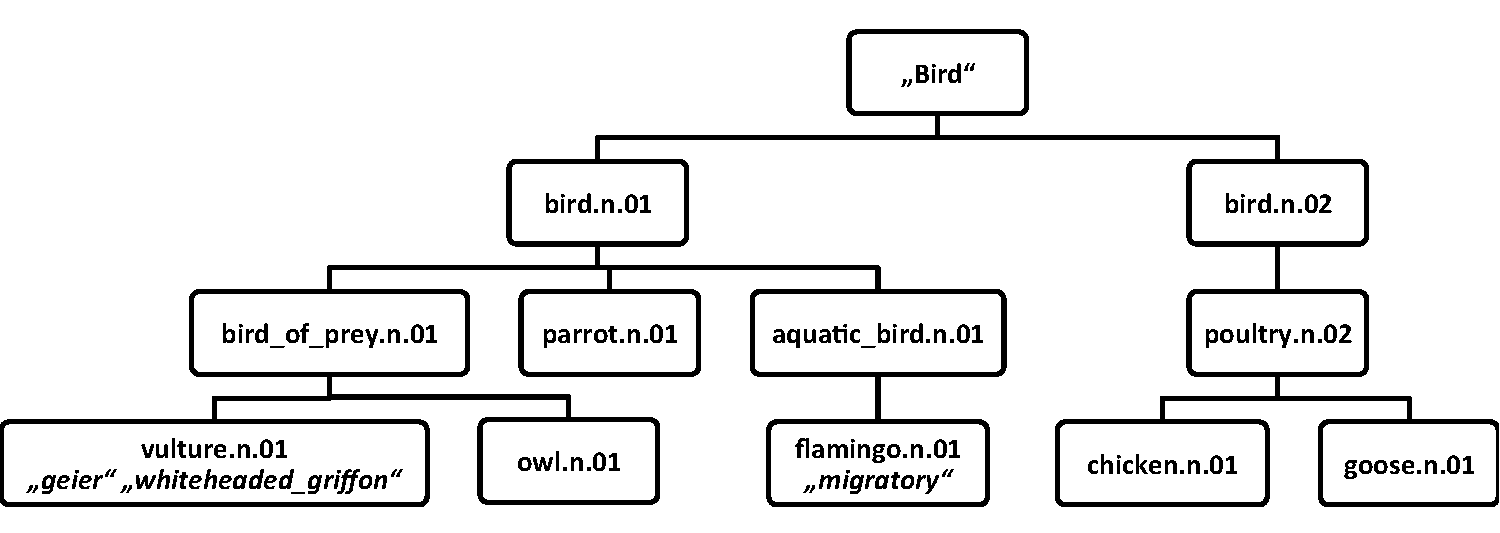
\includegraphics[width=\textwidth]{images/searchtree.pdf}
\caption{Examplary searchtree (excerpt) for search term ``bird''}
\label{fig_searchtree}
\end{figure}

The same figure also visualizes that a searchtree is a tree of specializations. These specializations are retrieved using WordNet's hypnoym relations\index{Hyponym}. For some terms, especially geographic Synsets, specializations are not applicable, so we use part-meronyms\index{Part-meronym} (part-of relationships), when no hyponyms are available.\\


Figure \ref{fig_nodestructure} shows the internal data structure of the tree. Each node represents one Synset, and references a list of more specific Synsets (\emph{hyponyms} or \emph{meronyms}). 

\begin{figure}[h]
\centering
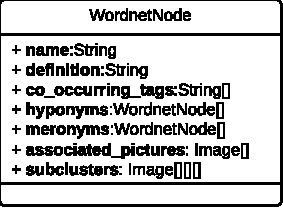
\includegraphics[]{images/wordnetnode_class_diagram.pdf}
\caption{Tree node data structure}
\label{fig_nodestructure}
\end{figure}


\subsection{Assigning Pictures to Tree Nodes}
\label{sec_picturestonodes}
Generally, assigning pictures to tree nodes is simple: Each node gets linked with all images that have been annotated with the Synset it represents during Synset detection. \\
In addition, strongly co-occurring tags are used for a higher recall. Co-occurring tags are those keywords that could not be mapped to any Synset. They may, however, be closely related to certain Synsets, with which they often occurr together. When that is the case, the keyword is added to the list of \emph{co\_occurring\_tags} of the node. \\
We define a \emph{strong} co-occurrence based on tf-idf \index{Tf-idf} values\todo{explain tf-idf}. If a simpler co-occurrence measure (e.g. the ratio of co-occurrences to the total number of occurrences of the term) was used, very common keywords like camera models would be strong co-occurrences with many Synsets despite the lack of an actual relation. \\
We observed that the co-occurring keywords can be useful to find terms in foreign languages and proper nouns, but of course also introduces noise. The key to the quality of this features is the choice of the threshold. Reasonably good results were achieved with $0.75 * max\_tf\_idf$, where $max\_tf\_idf$ is the maximal score across all values. \\

After adding all pictures that are annotated with the Synset itself or one of the related tags to the node's \emph{associated\_pictures}, some nodes may only have one or very few images. To create a balanced result with image sets of a significant size, nodes considered too small are merged into their parent node. Whether a node is too small is determined by the parameter \emph{minimal\_node\_size}, which states the minimal number of images a node must have. To avoid merging of small nodes completely, the parameter should be set to 0.\\ 
The merge process is simple: All associated pictures of the node are unioned into the parent node's pictures and the node itself deleted. \todo{What happens when subnodes exist?}
